\documentclass[12pt]{article}

%%%%%%%%%%%%%%%%%%%%%%%%%%%%%%%%%%%%%%%%%%%%%
%%%%%%%%%%%%%%%% PACKAGES %%%%%%%%%%%%%%%%%%%
%%%%%%%%%%%%%%%%%%%%%%%%%%%%%%%%%%%%%%%%%%%%%

\usepackage[inner=2.1cm, bottom=1.5cm, top=1.5cm, outer=2.1cm,
  headheight=24pt, % as per the warning by fancyhdr
  includehead,includefoot,
  heightrounded]{geometry}
% Set the font
\usepackage{helvet}
\renewcommand{\familydefault}{\sfdefault}
% bitfield
\usepackage{bytefield}
% urls
\usepackage[hidelinks]{hyperref}
% disable indent
\usepackage[skip=1em, indent=0pt]{parskip}
% shifted environment
\newenvironment{content}%
  {\list{}{\leftmargin=2cm}\item[]}%
  {\endlist}
% cell color
\usepackage[table, dvipsnames]{xcolor}
% drawings
\usepackage{tikz}
\usepackage{pgfplots}
\pgfplotsset{compat=1.18}
\usetikzlibrary{shapes.geometric,angles,quotes}
\usetikzlibrary{arrows.meta}
\usetikzlibrary{positioning}
\usetikzlibrary{babel}
\usetikzlibrary{fit}
\usetikzlibrary{angles, quotes}
\tikzset{
% Define standard arrow tip
>={Latex[scale=1.25]}
}
\usepackage{tikz-layers}
% floating figures
\usepackage{float}
% do computations
\usepackage{calc}
% advanced tables
\usepackage{makecell}
\usepackage{tabularx}
\newcolumntype{Y}{>{\centering\arraybackslash}X}
\usepackage{multirow}
\usepackage{graphicx}
% no title at the end of pages
\usepackage[nobottomtitles]{titlesec}

%%%%%%%%%%%%%%%%%%%%%%%%%%%%%%%%%%%%%%%%%%%%%%
%%%%%%%%%%%%%%%% Variables %%%%%%%%%%%%%%%%%%%
%%%%%%%%%%%%%%%%%%%%%%%%%%%%%%%%%%%%%%%%%%%%%%

% VARIABLES
\def\version{DRAFT-1.0.0}
\def\parent{Educational Computer Architecture Platform 5}
\def\project{ECAP5-DPROC RISC-V processor}
\def\title{Architecture Document}


%%%%%%%%%%%%%%%%%%%%%%%%%%%%%%%%%%%%%%%%%%%%%%%%%%
%%%%%%%%%%%%%%%% Configuration %%%%%%%%%%%%%%%%%%%
%%%%%%%%%%%%%%%%%%%%%%%%%%%%%%%%%%%%%%%%%%%%%%%%%%

\setlength{\tabcolsep}{10pt}
\renewcommand{\arraystretch}{1.5}
% Functional requirement environment
\newlength{\reqtablelength}
\setlength{\reqtablelength}{0.85\textwidth}
\newcommand{\reqcolor}{blue!20!gray}
\newcommand{\req}[3]{
  \begin{center}
  {
    \footnotesize
    \begin{tabularx}{\reqtablelength}{|l|X|}
      \hline
      \cellcolor{\reqcolor!30}\textbf{ID} & #1\\
      \hline
      \cellcolor{\reqcolor!15}\textbf{Description} & \cellcolor{\reqcolor!5}{#2} \\
      \hline
      \cellcolor{\reqcolor!15}\textbf{Refers to} & \cellcolor{\reqcolor!5}\makecell[l]{#3} \\
      \hline
    \end{tabularx}
  }
  \end{center}
}
\newcommand{\reqwithratio}[4]{
  \begin{center}
  {
    \footnotesize
    \begin{tabularx}{\reqtablelength}{|l|X|}
      \hline
      \cellcolor{\reqcolor!30}\textbf{ID} & #1\\
      \hline
      \cellcolor{\reqcolor!15}\textbf{Description} & \cellcolor{\reqcolor!5}{#2} \\
      \hline
      \cellcolor{\reqcolor!15}\textbf{Rationale} & \cellcolor{\reqcolor!5}#3 \\
      \hline
      \cellcolor{\reqcolor!15}\textbf{Refers to} & \cellcolor{\reqcolor!5}#4 \\
      \hline
    \end{tabularx}
  }
  \end{center}
}
% User requirement 
\newlength{\ureqtablelength}
\setlength{\ureqtablelength}{0.85\textwidth}
\newcommand{\ureqcolor}{blue!20!gray}
\newcommand{\ureq}[2]{
  \begin{center}
  {
    \footnotesize
    \begin{tabularx}{\ureqtablelength}{|l|X|}
      \hline
      \cellcolor{\ureqcolor!30}\textbf{ID} & #1\\
      \hline
      \cellcolor{\ureqcolor!15}\textbf{Description} & \cellcolor{\ureqcolor!5}#2 \\
      \hline
    \end{tabularx}
  }
  \end{center}
}
% External interface requirement
\newlength{\ireqtablelength}
\setlength{\ireqtablelength}{0.85\textwidth}
\newcommand{\ireqcolor}{blue!20!gray}
\newcommand{\ireq}[3]{
  \begin{center}
  {
    \footnotesize
    \begin{tabularx}{\ireqtablelength}{|l|X|}
      \hline
      \cellcolor{\ireqcolor!30}\textbf{ID} & #1\\
      \hline
      \cellcolor{\ireqcolor!15}\textbf{Description} & \cellcolor{\ireqcolor!5}#2 \\
      \hline
      \cellcolor{\ireqcolor!15}\textbf{Refers to} & \cellcolor{\ireqcolor!5}\makecell[l]{#3} \\
      \hline
    \end{tabularx}
  }
  \end{center}
}
\newcommand{\ireqwithratio}[4]{
  \begin{center}
  {
    \footnotesize
    \begin{tabularx}{\ireqtablelength}{|l|X|}
      \hline
      \cellcolor{\ireqcolor!30}\textbf{ID} & #1\\
      \hline
      \cellcolor{\ireqcolor!15}\textbf{Description} & \cellcolor{\ireqcolor!5}#2 \\
      \hline
      \cellcolor{\ireqcolor!15}\textbf{Rationale} & \cellcolor{\ireqcolor!5}\makecell[l]{#3} \\
      \hline
      \cellcolor{\ireqcolor!15}\textbf{Refers to} & \cellcolor{\ireqcolor!5}\makecell[l]{#4} \\
      \hline
    \end{tabularx}
  }
  \end{center}
}

% Configure headers and footers
\usepackage{fancyhdr}
\renewcommand{\headrulewidth}{1pt}
\renewcommand{\footrulewidth}{1pt}
\renewcommand{\headruleskip}{4pt}
\renewcommand{\footruleskip}{4pt}
\fancyhead{}\fancyfoot{}
\fancyhead[HL]{\scriptsize{\textbf{\parent} \\
\project}}
\fancyhead[HR]{\scriptsize{Page \thepage \\
}}
\fancyfoot[FL]{\scriptsize{\title}}
\fancyfoot[FR]{\scriptsize{Issue Date: \today}}
\fancyfoot[FC]{\scriptsize{\vspace{1em}\textit{Revision \version}}}

%%%%%%%%%%%%%%%%%%%%%%%%%%%%%%%%%%%%%%%%%%%%
%%%%%%%%%%%%%%%% Content %%%%%%%%%%%%%%%%%%%
%%%%%%%%%%%%%%%%%%%%%%%%%%%%%%%%%%%%%%%%%%%%

\begin{document}
\begin{titlepage}

\large{\textbf{ECAP5-DPROC}}

\vspace{-0.5em}

\normalsize{RISC-V processor}

\vspace{1.5em}

\Huge{\textbf{Architecture Document}}

\normalsize{\textbf{Revision: \version}}

\normalsize{\textbf{Issue Date: \today}}

\vspace*{\fill}

{\scriptsize \parindent0pt \itshape
Copyright (C) Clément Chaine

ECAP5-DPROC is free software: you can redistribute it and/or modify it under the terms of the GNU General Public License as published by the Free Software Foundation, either version 3 of the License, or (at your option) any later version.

ECAP5-DPROC is distributed in the hope that it will be useful, but WITHOUT ANY WARRANTY; without even the implied warranty of MERCHANTABILITY or FITNESS FOR A PARTICULAR PURPOSE. See the GNU General Public License for more details.

\vspace{-0.5em}

You should have received a copy of the GNU General Public License along with ECAP5-DPROC. If not, see \textnormal{\url{http://www.gnu.org/licenses/}}}

\vspace{1em}

\par\noindent\rule{\textwidth}{1pt}

\end{titlepage}

\newpage

\pagestyle{fancy}
\normalsize
\tableofcontents
\newpage
\section{Introduction}
\subsection{Purpose}

\begin{content}
This documents aims at defining the requirements for ECAP5-DPROC as well as describing its architecture. Both user and product requirements will be covered.
\end{content}

\subsection{Intended Audience and Use}

\begin{content}
This document targets hardware engineers who shall implement ECAP5-DPROC by refering to the described architecture. It is also intended for system engineers working on the integration of ECAP5-DPROC in ECAP5. Finally, this document shall be used as a technical reference by software engineers configuring ECAP5-DPROC through hardware-software interfaces.
\end{content}

\subsection{Product Scope}

\begin{content}
  ECAP5-DPROC is an implementation of the RISC-V instruction set architecture targetting \textit{Educational Computer Architecture Platform 5} (ECAP5). It will provide the main means of software execution in ECAP5.
\end{content}

\subsection{Conventions}

Requirements shall be described here.

Requirement relationships :
\begin{itemize}
    \item Composition
    \item Derivation
    \item Refinement
    \item Satisfy
    \item Verify
    \item Copy
\end{itemize}

The bit indexing shall be described somewhere.

Byte size as well.

Inputs missing from timing diagrams are considered low or undefined.

Italic names are timing diagram parameters.

\subsection{Definitions and Abbreviations}

hardware-configurable

software-configurable

\subsection{References}

\begin{center}
{
  \vspace{0.5em}
  \small
  \begin{tabularx}{0.9\textwidth}{|c|c|X|}
    \hline
    \cellcolor{gray!20}\textbf{Date} & \cellcolor{gray!20}\textbf{Version} & \cellcolor{gray!20}\textbf{Title} \\
    \hline
    December 13, 2019 & 20191213 & The RISC-V Instruction Set Manual Volume I: User-Level ISA \\
    \hline
    March 22, 2019 & 0.13.2 & RISC-V External Debug Support \\
    \hline
    June 22, 2010 & B.4 & WISHBONE System-on-Chip (SoC) Interconnection Architecture for Portable IP Cores \\
    \hline
%    \hline
  \end{tabularx}
  \vspace{0.5em}
}
\end{center}

\newpage

\section{Overall Description}

\subsection{User needs}

\begin{content}
ECAP5 is the primary user for ECAP5-DPROC. ECAP5-DPROC could however be used as a standalone RISC-V processor. The following requirements define the user needs. 
\end{content}

\ureq{U\_INSTRUCTION\_SET\_01}{
  ECAP5-DPROC shall implement the RV32I instruction set.
}

\begin{content}
  In order to improve the usability of ECAP5-DPROC, it shall have a \textit{von Neumann} architecture as it only requires one memory interface.
\end{content}

\ureq{U\_MEMORY\_INTERFACE\_01}{
  ECAP5-DPROC shall access both instructions and data through a unique memory interface.
}

\ureq{U\_MEMORY\_INTERFACE\_02}{
  ECAP5-DPROC's unique memory interface shall be compliant with the AXI-Lite specification.
}

\ureq{U\_RESET\_01}{
  ECAP5-DPROC shall provide a signal which shall hold ECAP5-DPROC in a reset state while asserted.
}

\begin{content}
The polarity of the reset signal mentionned in \texttt{U\_RESET\_01} is not specified by the user.
\end{content}

\ureq{U\_BOOT\_ADDRESS\_01}{
  The address at which ECAP5-DPROC jumps after the reset signal is deasserted shall be hardware-configurable.
}

\begin{content}
The address mentionned in \texttt{U\_BOOT\_ADDRESS\_01} can be either configured through hardware signals or can be selected at compile-time.
\end{content}

\ureq{U\_HARDWARE\_INTERRUPT\_01}{
  ECAP5-DPROC shall provide an signal which shall interrupt ECAP5-DPROC's execution flow while asserted.
}

\ureq{U\_HARDWARE\_INTERRUPT\_02}{
  ECAP5-DPROC shall jump to a software-configurable address when it is interrupted.
}

\begin{content}
The memory address at which ECAP5-DPROC shall jump to when interrupted is not specified by the user.
\end{content}

\ureq{U\_DEBUG\_01}{
  ECAP5-DPROC shall be compliant with the RISC-V External Debug Support specification.
}

\begin{content}
There is no performance goal required by ECAP5 for ECAP5-DPROC as ECAP5 is an educational platform.
\end{content}

\subsection{Assumptions and Dependencies}

\begin{content}
Describe what the assumptions for the product are : Targeting the ecp5 family, based around opensource toolchains.
\end{content}

\section{Requirements}

\subsection{External Interface Requirements}

\begin{figure}[h!]
    \centering
    \scalebox{0.85}{
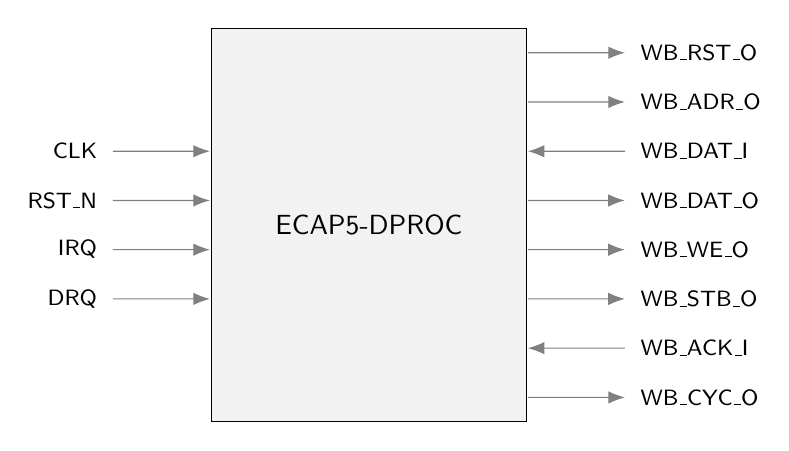
\begin{tikzpicture}[scale=1.25, draw=gray, inner sep=0, outer sep=0]
  \node[rectangle, draw=black,
    minimum height = 5cm,
    minimum width = 4cm,
    fill = gray!10] (box) at (0, 0) {ECAP5-DPROC};

  % left
  \node (lport1) at ([yshift=0.75cm]box.west) {};
  \node (lport2) at ([yshift=0.25cm]box.west) {};
  \node (lport3) at ([yshift=-0.25cm]box.west) {};
  \node (lport4) at ([yshift=-0.75cm]box.west) {};

  \draw[->] ([xshift=-1cm]lport1.center) node[left=0.2cm, anchor=east]{\footnotesize CLK} -- (lport1);
  \draw[->] ([xshift=-1cm]lport2.center) node[left=0.2cm, anchor=east]{\footnotesize RST\_N} -- (lport2);
  \draw[->] ([xshift=-1cm]lport3.center) node[left=0.2cm, anchor=east]{\footnotesize IRQ} -- (lport3);
  \draw[->] ([xshift=-1cm]lport4.center) node[left=0.2cm, anchor=east]{\footnotesize DRQ} -- (lport4);

  % right
  \node (rport4) at ([yshift=0.25cm]box.east) {};
  \node (rport3) at ([yshift=0.5cm]rport4.center) {};
  \node (rport2) at ([yshift=0.5cm]rport3.center) {};
  \node (rport1) at ([yshift=0.5cm]rport2.center) {};

  \node (rport5) at ([yshift=-0.25cm]box.east) {};
  \node (rport6) at ([yshift=-0.5cm]rport5.center) {};
  \node (rport7) at ([yshift=-0.5cm]rport6.center) {};
  \node (rport8) at ([yshift=-0.5cm]rport7.center) {};

  \draw[<-] ([xshift=1cm]rport1.center) node[right=0.2cm, anchor=west]{\footnotesize WB\_RST\_O} -- (rport1);
  \draw[<-] ([xshift=1cm]rport2.center) node[right=0.2cm, anchor=west]{\footnotesize WB\_ADR\_O} -- (rport2);
  \draw[->] ([xshift=1cm]rport3.center) node[right=0.2cm, anchor=west]{\footnotesize WB\_DAT\_I} -- (rport3);
  \draw[<-] ([xshift=1cm]rport4.center) node[right=0.2cm, anchor=west]{\footnotesize WB\_DAT\_O} -- (rport4);
  \draw[<-] ([xshift=1cm]rport5.center) node[right=0.2cm, anchor=west]{\footnotesize WB\_WE\_O} -- (rport5);
  \draw[<-] ([xshift=1cm]rport6.center) node[right=0.2cm, anchor=west]{\footnotesize WB\_STB\_O} -- (rport6);
  \draw[->] ([xshift=1cm]rport7.center) node[right=0.2cm, anchor=west]{\footnotesize WB\_ACK\_I} -- (rport7);
  \draw[<-] ([xshift=1cm]rport8.center) node[right=0.2cm, anchor=west]{\footnotesize WB\_CYC\_O} -- (rport8);
\end{tikzpicture}
}

    \caption{Schematic view of the external interface of ECAP5-DPROC}
    \label{fig:externalinterface}
\end{figure}

\begin{table}[H]
  \centering
  {
\footnotesize
\begin{tabularx}{0.9\textwidth}{|l|c|c|X|}
  \hline
  \cellcolor{gray!20}\textbf{NAME} & \cellcolor{gray!20}\textbf{TYPE} & \cellcolor{gray!20}\textbf{WIDTH} & \cellcolor{gray!20}\textbf{DESCRIPTION} \\
  \hline
  CLK & I & 1 & Clock input. \\
  \hline
  RST\_N & I & 1 & Hardware reset. Active low. \\
  \hline
  IRQ & I & 1 & External interrupt request. \\
  \hline
  DRQ & I & 1 & Debug request. \\
  \hline
\end{tabularx}
}

  \caption{ECAP5-DPROC control signals}
  \label{tab:control-interface}
\end{table}

\begin{table}[H]
  \centering
  {
\footnotesize
\begin{tabularx}{0.9\textwidth}{|l|c|c|X|}
  \hline
  \cellcolor{gray!20}\textbf{NAME} & \cellcolor{gray!20}\textbf{TYPE} & \cellcolor{gray!20}\textbf{WIDTH} & \cellcolor{gray!20}\textbf{DESCRIPTION} \\
  \hline
  \multicolumn{4}{|l|}{\textbf{READ ADDRESS BUS}} \\
  \hline
  ARADDR & O & 32 & Read address. \\
  \hline
  ARVALID & O & 1 & Read address valid. \\
  \hline
  ARREADY & I & 1 & Read address ready. \\ 
  \hline
  \multicolumn{4}{|l|}{\textbf{READ DATA BUS}} \\
  \hline
  RDATA & I & 32 & Read data. \\
  \hline
  RRESP & I & 2 & Read response. \\
  \hline
  RVALID & I & 1 & Read valid. \\
  \hline
  RREADY & O & 1 & Read ready. \\ 
  \hline
  \multicolumn{4}{|l|}{\textbf{WRITE ADDRESS BUS}} \\
  \hline
  AWADDR & O & 32 & Write address. \\
  \hline
  AWVALID & O & 1 & Write address valid. \\
  \hline
  AWREADY & I & 1 & Write address ready \\
  \hline
  \multicolumn{4}{|l|}{\textbf{WRITE DATA BUS}} \\
  \hline
  WDATA & O & 32 & Write data. \\
  \hline
  WSTRB & O & 4 & Write strobes. \\
  \hline
  \multicolumn{4}{|l|}{\textbf{WRITE RESPONSE BUS}} \\
  \hline
  BRESP & I & 2 & Write response. \\
  \hline
  BVALID & I & 1 & Write response valid. \\
  \hline
  BREADY & O & 1 & Response ready. \\
  \hline
\end{tabularx}
}

  \caption{ECAP5-DPROC memory interface signals}
  \label{tab:memory-interface}
\end{table}

\ireq{I\_CLK\_01}{
  All inputs and outputs of ECAP5-DPROC shall belong to CLK's clock domain.
}{}

\ireq{I\_RESET\_01}{
  The RST\_N signal shall hold ECAP5-DPROC in a reset state while asserted.
}{
  U\_RESET\_01
}

\ireq{I\_RESET\_02}{
  RST\_N polarity shall be active low.
}{}

\ireq{I\_IRQ\_01}{
  ECAP5-DPROC shall jump to a software-configurable address when input IRQ is asserted.
}{
  U\_HARDWARE\_INTERRUPT\_01, U\_HARDWARE\_INTERRUPT\_02
}

\ireq{I\_DIRQ\_01}{
  TBD
}{}

\ireq{I\_MEMORY\_INTERFACE\_01}{
  Signals from table \ref{tab:memory-interface} shall be compliant with the AXI-Lite specification.
}{
  U\_MEMORY\_INTERFACE\_02
}

\begin{content}
  Behavioral specification for symbols in table \ref{tab:memory-interface} is outlined in the functional requirements section, subsection \ref{spec-memory-interface}.
\end{content}

\subsection{Functional Requirements}

\subsubsection{Register file}

\req{F\_REGISTERS\_01}{
  ECAP5-DPROC shall implement 31 user-accessible general purpose registers ranging from \texttt{x0} to \texttt{x31}.
}{U\_INSTRUCTION\_SET\_01}

\req{F\_REGISTERS\_02}{
  Register \texttt{x0} shall be hardwired to the constant zero.
}{U\_INSTRUCTION\_SET\_01}

\req{F\_REGISTERS\_03}{
  ECAP5-DPROC shall implement a \texttt{pc} user-accessible register storing the address of the current instruction.
}{U\_INSTRUCTION\_SET\_01}

\subsubsection{Instruction decoding}

\begin{content}
  Figure \ref{fig:instructionencoding} outlines the different instruction encodings for the RV32I instruction set. The \texttt{opcode} parameter is a unique identifier for each instruction. The instruction encoding is infered from the opcode as there can only be one encoding per opcode.
\end{content}

\begin{figure}[h!]
    \centering
    \vspace{0.5em}

\hspace{2em}
\scalebox{0.9}{
\begin{bytefield}[
    bitwidth=1.1em, 
    endianness=big, 
    bitformatting={\scriptsize}, 
    boxformatting={\centering\footnotesize\ttfamily},
    rightcurly=., rightcurlyspace=5pt
]{32}
  \bitheader{0,6,7,8,11,12,14,15,19,20,24,25,31} \\
  \begin{rightwordgroup}{\footnotesize R-type}
    \bitbox{7}{funct7}
    \bitbox{5}{rs2}
    \bitbox{5}{rs1}
    \bitbox{3}{func3}
    \bitbox{5}{rd}
    \bitbox{7}{opcode}
  \end{rightwordgroup}
  \\[2ex]
  \begin{rightwordgroup}{\footnotesize I-type}
    \bitbox{12}{imm[11:0]}
    \bitbox{5}{rs1}
    \bitbox{3}{func3}
    \bitbox{5}{rd}
    \bitbox{7}{opcode}
  \end{rightwordgroup}
  \\[2ex]
  \begin{rightwordgroup}{\footnotesize S-type}
    \bitbox{7}{imm[11:5]}
    \bitbox{5}{rs2}
    \bitbox{5}{rs1}
    \bitbox{3}{func3}
    \bitbox{5}{imm[4:0]}
    \bitbox{7}{opcode}
  \end{rightwordgroup}
  \\[2ex]
  \begin{rightwordgroup}{\footnotesize B-type}
    \bitbox{1}{a}
    \bitbox{6}{imm[10:5]}
    \bitbox{5}{rs2}
    \bitbox{5}{rs1}
    \bitbox{3}{func3}
    \bitbox{4}{imm[4:1]}
    \bitbox{1}{b}
    \bitbox{7}{opcode}
  \end{rightwordgroup}
  \\[2ex]
  \begin{rightwordgroup}{\footnotesize U-type}
    \bitbox{20}{imm[31:12]}
    \bitbox{5}{rd}
    \bitbox{7}{opcode}
  \end{rightwordgroup}
  \\[2ex]
  \begin{rightwordgroup}{\footnotesize J-type}
    \bitbox{1}{c}
    \bitbox{10}{imm[10:1]}
    \bitbox{1}{b}
    \bitbox{8}{imm[31:12]}
    \bitbox{5}{rd}
    \bitbox{7}{opcode}
  \end{rightwordgroup}
\end{bytefield}
}

\vspace{0.25em}
\scalebox{0.7}{
\begin{tabularx}{0.8\textwidth}{Y Y Y}
a: \texttt{imm[12]} & b: \texttt{imm[11]} & c: \texttt{imm[20]}
\end{tabularx}
}

    \caption{Instruction encodings of the RV32I instruction set}
    \label{fig:instructionencoding}
\end{figure}

\paragraph{Immediate encoding}

\begin{content}
  Only one immediate value can be encoded in one instruction. The value can be reconstructed from fragments of the following format : imm[x] representing the x\textsuperscript{th} bit or imm[x:y] representing bits from the x\textsuperscript{th} to the y\textsuperscript{th} both included.
\end{content}

\req{F\_INSTR\_IMMEDIATE\_01}{
  Immediate values shall be sign-extended.
}{U\_INSTRUCTION\_SET\_01}

\req{F\_INSTR\_IMMEDIATE\_02}{
  The value of an instruction immediate shall be the concatenation of immediate fragments from the instruction encoding.
}{U\_INSTRUCTION\_SET\_01}

\req{F\_INSTR\_IMMEDIATE\_03}{
  Missing immediate fragments shall be replaced by zeros.
}{U\_INSTRUCTION\_SET\_01}

\begin{content}
  RV32I is called a Load/Store ISA, meaning that instructions inputs and outputs are passed through registers or through an instruction immediate. There are specific instructions for loading and storing data into memory.
\end{content}

\paragraph{Instruction inputs}

\req{F\_INSTR\_FIRST\_INPUT\_01}{
  Instructions encoded using the R-type, I-type, S-type and B-type shall take as their first input the value stored in the register designated by the \texttt{rs1} parameter.
}{U\_INSTRUCTION\_SET\_01}

\req{F\_INSTR\_FIRST\_INPUT\_02}{
  Instructions encoded using the U-type and J-type shall take as their first input the immediate value encoded in the instruction.
}{U\_INSTRUCTION\_SET\_01}

\req{F\_INSTR\_SECOND\_INPUT\_01}{
  Instructions encoded using the R-type, S-type and B-type shall take as their second input the value stored in the register designated by the \texttt{rs2} parameter.
}{U\_INSTRUCTION\_SET\_01}

\req{F\_INSTR\_SECOND\_INPUT\_02}{
  Instructions encoded using the I-type shall take as its second input the immediate value encoded in the instruction.
}{U\_INSTRUCTION\_SET\_01}

\req{F\_INSTR\_THIRD\_INPUT\_01}{
  Instructions encoded using the S-type and B-type shall take as their third input the immediate value encoded in the instruction.
}{U\_INSTRUCTION\_SET\_01}

\paragraph{Instruction outputs}

\req{F\_INSTR\_OUTPUT\_01}{
  Instructions encoded using the R-type, I-type, U-type and J-type shall store their result in the register designated by the \texttt{rd} parameter.
}{U\_INSTRUCTION\_SET\_01}

\req{F\_INSTR\_OUTPUT\_02}{
  Instructions encoded using the S-type and B-type do not produce any result.
}{U\_INSTRUCTION\_SET\_01}

\paragraph{Instruction variants}

\req{F\_INSTR\_VARIANT\_01}{
  Instructions encoded using the R-type, I-type, S-type and B-type shall use the \texttt{func3} parameter as a behavior variant selector.
}{U\_INSTRUCTION\_SET\_01}

\req{F\_INSTR\_VARIANT\_02}{
  Instructions encoded using the R-type shall use the \texttt{func7} parameter as a secondary behavior variant selector.
}{U\_INSTRUCTION\_SET\_01}

\paragraph{Opcodes}

\vspace{1em}
\begin{content}
  Table \ref{tab:opcodemap} outlines the different opcodes values of the RV32I instruction set. Cells marked as \textit{noimp} are for opcodes that are not implemented in ECAP5-DPROC.
\end{content}

\begin{table}[H]
  \centering
  \scalebox{0.8}{
\footnotesize
\begin{tabular}{|r|c|c|c|c|c|c|c|c|}
  \hline
  opcode[1:0] & \multicolumn{8}{|c|}{11} \\
  \hline
  opcode[4:2] & \multirow{2}{*}{000} & \multirow{2}{*}{001} & \multirow{2}{*}{010} & \multirow{2}{*}{011} & \multirow{2}{*}{100} & \multirow{2}{*}{101} & \multirow{2}{*}{110} & \multirow{2}{*}{111} \\
  \cline{1-1}
  opcode[6:5] & & & & & & & & \\
  \hline
  00 & LOAD & \cellcolor{gray!20}\textit{noimp} & \cellcolor{gray!20}\textit{noimp} & MISC-MEM & OP-IMM & AUIPC & \cellcolor{gray!20}\textit{noimp} & \cellcolor{gray!20}\textit{noimp} \\
  \hline
  01 & STORE & \cellcolor{gray!20}\textit{noimp} & \cellcolor{gray!20}\textit{noimp} & \cellcolor{gray!20}\textit{noimp} & OP & LUI & \cellcolor{gray!20}\textit{noimp} & \cellcolor{gray!20}\textit{noimp} \\
  \hline
  10 & \cellcolor{gray!20}\textit{noimp} & \cellcolor{gray!20}\textit{noimp} & \cellcolor{gray!20}\textit{noimp} & \cellcolor{gray!20}\textit{noimp} & \cellcolor{gray!20}\textit{noimp} & \cellcolor{gray!20}\textit{noimp} & \cellcolor{gray!20}\textit{noimp} & \cellcolor{gray!20}\textit{noimp} \\
  \hline
  11 & BRANCH & JALR & \cellcolor{gray!20}\textit{noimp} & JAL & SYSTEM & \cellcolor{gray!20}\textit{noimp} & \cellcolor{gray!20}\textit{noimp} & \cellcolor{gray!20}\textit{noimp} \\
  \hline
\end{tabular}
}

  \caption{Opcode values for the RV32I instruction set.}
  \label{tab:opcodemap}
\end{table}

\req{F\_OPCODE\_ENCODING\_01}{
  Instructions which use the LUI opcode shall be decoded as an U-type instruction.
}{U\_INSTRUCTION\_SET\_01}

\req{F\_OPCODE\_ENCODING\_02}{
  Instructions which use the AUIPC opcode shall be decoded as an U-type instruction.
}{U\_INSTRUCTION\_SET\_01}

\req{F\_OPCODE\_ENCODING\_03}{
  Instructions which use the JAL opcode shall be decoded as a J-type instruction.
}{U\_INSTRUCTION\_SET\_01}

\req{F\_OPCODE\_ENCODING\_04}{
  Instructions which use the JALR opcode shall be decoded as an I-type instruction.
}{U\_INSTRUCTION\_SET\_01}

\req{F\_OPCODE\_ENCODING\_05}{
  Instructions which use the BRANCH opcode shall be decoded as a B-type instruction.
}{U\_INSTRUCTION\_SET\_01}

\req{F\_OPCODE\_ENCODING\_06}{
  Instructions which use the LOAD opcode shall be decoded as an I-type instruction.
}{U\_INSTRUCTION\_SET\_01}

\req{F\_OPCODE\_ENCODING\_07}{
  Instructions which use the STORE opcode shall be decoded as a S-type instruction.
}{U\_INSTRUCTION\_SET\_01}

\req{F\_OPCODE\_ENCODING\_08}{
  Instructions which use the OP-IMM opcode shall be decoded as an I-type instruction.
}{U\_INSTRUCTION\_SET\_01}

\req{F\_OPCODE\_ENCODING\_09}{
  Instructions which use the OP opcode shall be decoded as a R-type instruction.
}{U\_INSTRUCTION\_SET\_01}

\req{F\_OPCODE\_ENCODING\_10}{
  Instructions which use the MISC-MEM opcode shall be decoded as an I-type instruction.
}{U\_INSTRUCTION\_SET\_01}

\req{F\_OPCODE\_ENCODING\_11}{
  Instructions which use the SYSTEM opcode shall be decoded as an I-type instruction.
}{U\_INSTRUCTION\_SET\_01}

\subsubsection{Instructions behaviors}

\paragraph{LUI}

\req{F\_LUI\_01}{
  The LUI behavior shall be applied when the opcode is LUI.
}{U\_INSTRUCTION\_SET\_01}

\reqwithratio{F\_ADDI\_02}{
  The output of LUI shall be the value of its first input.
}{
  The LUI instruction shall load the 20 upper bits of the instruction immediate into the destination register and fill the remaining bits with zeros. This is the default behavior for instruction immediates as stated in F\_INSTR\_IMMEDIATE\_02 and F\_INSTR\_IMMEDIATE\_03.
}{U\_INSTRUCTION\_SET\_01}

\paragraph{AUIPC}

\req{F\_AUIPC\_01}{
  The AUIPC behavior shall be applied when the opcode is AUIPC.
}{U\_INSTRUCTION\_SET\_01}

\req{F\_AUIPC\_02}{
  The output of AUIPC shall be the sum of its first input and the address of the AUIPC instruction.
}{U\_INSTRUCTION\_SET\_01}

\begin{content}
Depending on implementation details, the address of the AUIPC instruction might be different from the address found in the \texttt{pc} register at the moment of executing the instruction behavior.
\end{content}

\paragraph{JAL}

\req{F\_JAL\_01}{
  The JAL behavior shall be applied when the opcode is JAL.
}{U\_INSTRUCTION\_SET\_01}

\req{F\_JAL\_02}{
  The \texttt{pc} register shall be updated with the sum of the address of the JAL instruction with its first input. 
}{U\_INSTRUCTION\_SET\_01}

\begin{content}
Depending on implementation details, the address of the JAL instruction might be different from the address found in the \texttt{pc} register at the moment of executing the instruction behavior.
\end{content}

\reqwithratio{F\_JAL\_03}{
  The output of JAL shall be the address of the JAL instruction incremented by 4.
}{
  The JAL instruction shall output the address to the following instruction for it to be used as a \textit{return address} in the case of a function call.
}{U\_INSTRUCTION\_SET\_01}

\paragraph{JALR}

\req{F\_JALR\_01}{
  The JALR behavior shall be applied when the opcode is JALR and func3 is 0x0.
}{U\_INSTRUCTION\_SET\_01}

\req{F\_JALR\_02}{
  The \texttt{pc} register shall be updated with the sum of the first and second inputs of the JALR instruction.
}{U\_INSTRUCTION\_SET\_01}

\reqwithratio{F\_JALR\_03}{
  The output of JALR shall be the address of the JALR instruction incremented by 4.
}{
  The JALR instruction shall output the address to the following instruction for it to be used as a \textit{return address} in the case of a function call.
}{U\_INSTRUCTION\_SET\_01}

\begin{content}
Depending on implementation details, the address of the JALR instruction might be different from the address found in the \texttt{pc} register at the moment of executing the instruction behavior.
\end{content}

\paragraph{BEQ}

\req{F\_BEQ\_01}{
  The BEQ behavior shall be applied when the opcode is BRANCH and func3 is 0x0.
}{U\_INSTRUCTION\_SET\_01}

\paragraph{BNE}

\req{F\_BNE\_01}{
  The BNE behavior shall be applied when the opcode is BRANCH and func3 is 0x1.
}{U\_INSTRUCTION\_SET\_01}

\paragraph{BLT}

\req{F\_BLT\_01}{
  The BLT behavior shall be applied when the opcode is BRANCH and func3 is 0x4.
}{U\_INSTRUCTION\_SET\_01}

\paragraph{BGE}

\req{F\_BGE\_01}{
  The BGE behavior shall be applied when the opcode is BRANCH and func3 is 0x5.
}{U\_INSTRUCTION\_SET\_01}

\paragraph{BLTU}

\req{F\_BLTU\_01}{
  The BLTU behavior shall be applied when the opcode is BRANCH and func3 is 0x6.
}{U\_INSTRUCTION\_SET\_01}

\paragraph{BGEU}

\req{F\_BGEU\_01}{
  The BGEU behavior shall be applied when the opcode is BRANCH and func3 is 0x7.
}{U\_INSTRUCTION\_SET\_01}

\paragraph{LB}

\req{F\_LB\_01}{
  The LB behavior shall be applied when the opcode is LOAD and func3 is 0x0.
}{U\_INSTRUCTION\_SET\_01}

\paragraph{LH}

\req{F\_LH\_01}{
  The LH behavior shall be applied when the opcode is LOAD and func3 is 0x1.
}{U\_INSTRUCTION\_SET\_01}

\paragraph{LW}

\req{F\_LW\_01}{
  The LW behavior shall be applied when the opcode is LOAD and func3 is 0x2.
}{U\_INSTRUCTION\_SET\_01}

\paragraph{LBU}

\req{F\_LBU\_01}{
  The LBU behavior shall be applied when the opcode is LOAD and func3 is 0x4.
}{U\_INSTRUCTION\_SET\_01}

\paragraph{LHU}

\req{F\_LHU\_01}{
  The LHU behavior shall be applied when the opcode is LOAD and func3 is 0x5.
}{U\_INSTRUCTION\_SET\_01}

\paragraph{SB}

\req{F\_SB\_01}{
  The SB behavior shall be applied when the opcode is STORE and func3 is 0x0.
}{U\_INSTRUCTION\_SET\_01}

\paragraph{SH}

\req{F\_SH\_01}{
  The SH behavior shall be applied when the opcode is STORE and func3 is 0x1.
}{U\_INSTRUCTION\_SET\_01}

\paragraph{SW}

\req{F\_SW\_01}{
  The SW behavior shall be applied when the opcode is STORE and func3 is 0x2.
}{U\_INSTRUCTION\_SET\_01}

\paragraph{ADDI}

\req{F\_ADDI\_01}{
  The ADDI behavior shall be applied when the opcode is OP-IMM and when func3 is 0x0.
}{U\_INSTRUCTION\_SET\_01}

\req{F\_ADDI\_02}{
  The output of ADDI shall be the signed integer sum of its two inputs.
}{U\_INSTRUCTION\_SET\_01}

\req{F\_ADDI\_03}{
  The output of ADDI shall be truncated to 32-bits.
}{U\_INSTRUCTION\_SET\_01}

\paragraph{SLTI}

\req{F\_SLTI\_01}{
  The SLTI behavior shall be applied when the opcode is OP-IMM and when func3 is 0x2.
}{U\_INSTRUCTION\_SET\_01}

\req{F\_SLTI\_02}{
  The output of SLTI shall be 1 when the signed value of its first input is lower that the signed value of its second input. It shall be 0 otherwise.
}{U\_INSTRUCTION\_SET\_01}

\paragraph{SLTIU}

\req{F\_SLTIU\_01}{
  The SLTIU behavior shall be applied when the opcode is OP-IMM and when func3 is 0x3.
}{U\_INSTRUCTION\_SET\_01}

\req{F\_SLTIU\_02}{
  The output of SLTI shall be 1 when the unsigned value of its first input is lower that the unsigned value of its second input. It shall be 0 otherwise.
}{U\_INSTRUCTION\_SET\_01}

\paragraph{XORI}

\req{F\_XORI\_01}{
  The XORI behavior shall be applied when the opcode is OP-IMM and when func3 is 0x4.
}{U\_INSTRUCTION\_SET\_01}

\req{F\_XORI\_02}{
  The output of XORI shall be the result of a bitwise xor between its two inputs.
}{U\_INSTRUCTION\_SET\_01}

\paragraph{ORI}

\req{F\_ORI\_01}{
  The ORI behavior shall be applied when the opcode is OP-IMM and when func3 is 0x6.
}{U\_INSTRUCTION\_SET\_01}

\req{F\_ORI\_02}{
  The output of ORI shall be the result of a bitwise or between its two inputs.
}{U\_INSTRUCTION\_SET\_01}

\paragraph{ANDI}

\req{F\_ANDI\_01}{
  The ANDI behavior shall be applied when the opcode is OP-IMM and when func3 is 0x7.
}{U\_INSTRUCTION\_SET\_01}

\req{F\_ANDI\_02}{
  The output of ANDI shall be the result of a bitwise and between its two inputs.
}{U\_INSTRUCTION\_SET\_01}

\paragraph{SLLI}

\req{F\_SLLI\_01}{
  The SLLI behavior shall be applied when the opcode is OP-IMM and func3 is 0x1.
}{U\_INSTRUCTION\_SET\_01}

\req{F\_SLLI\_02}{
  The output of SLLI shall be its first input shifted left by the amount specified by the first 5 bits of its second input.
}{U\_INSTRUCTION\_SET\_01}

\req{F\_SLLI\_03}{
  Zeros shall be inserted in the lower bits when shifting.
}{U\_INSTRUCTION\_SET\_01}

\paragraph{SRLI}

\req{F\_SRLI\_01}{
  The SRLI behavior shall be applied when the opcode is OP-IMM, func3 is 0x5 and the 30\textsuperscript{th} bit of its second input is 0.
}{U\_INSTRUCTION\_SET\_01}

\req{F\_SRLI\_02}{
  The output of SRLI shall be its first input shifted right by the amount specified by the first 5 bits of its second input.
}{U\_INSTRUCTION\_SET\_01}

\req{F\_SRLI\_03}{
  Zeros shall be inserted in the upper bits when shifting.
}{U\_INSTRUCTION\_SET\_01}

\paragraph{SRAI}

\req{F\_SRAI\_01}{
  The SRAI behavior shall be applied when the opcode is OP-IMM, func3 is 0x5 and the 30\textsuperscript{th} bit of its second input is 1.
}{U\_INSTRUCTION\_SET\_01}

\req{F\_SRAI\_02}{
  The output of SRAI shall be its first input shifted right by the amount specified by the first 5 bits of its second input.
}{U\_INSTRUCTION\_SET\_01}

\req{F\_SRAI\_03}{
  The most significant bit of the first input shall be inserted in the upper bits when shifting.
}{U\_INSTRUCTION\_SET\_01}

\paragraph{ADD}

\req{F\_ADD\_01}{
  The ADD behavior shall be applied when the opcode is OP, func3 is 0x0 and the 30\textsuperscript{th} bit of its second input is 0.
}{U\_INSTRUCTION\_SET\_01}

\req{F\_ADD\_02}{
  The output of ADD shall be the signed integer sum of its two inputs.
}{U\_INSTRUCTION\_SET\_01}

\req{F\_ADD\_03}{
  The output of ADD shall be truncated to 32-bits.
}{U\_INSTRUCTION\_SET\_01}

\paragraph{SUB}

\req{F\_SUB\_01}{
  The SUB behavior shall be applied when the opcode is OP, func3 is 0x0 and the 30\textsuperscript{th} bit of its second input is 1.
}{U\_INSTRUCTION\_SET\_01}

\req{F\_SUB\_02}{
  The output of SUB shall be the signed integer difference of its first input minus its second input.
}{U\_INSTRUCTION\_SET\_01}

\req{F\_SUB\_03}{
  The output of SUB shall be truncated to 32-bits.
}{U\_INSTRUCTION\_SET\_01}

\paragraph{SLL}

\req{F\_SLL\_01}{
  The SLL behavior shall be applied when the opcode is OP and func3 is 0x1.
}{U\_INSTRUCTION\_SET\_01}

\req{F\_SLL\_02}{
  The output of SLL shall be its first input shifted left by the amount specified by the first 5 bits of its second input.
}{U\_INSTRUCTION\_SET\_01}

\req{F\_SLL\_03}{
  Zeros shall be inserted in the lower bits when shifting.
}{U\_INSTRUCTION\_SET\_01}

\paragraph{SLT}

\req{F\_SLT\_01}{
  The SLT behavior shall be applied when the opcode is OP and func3 is 0x2.
}{U\_INSTRUCTION\_SET\_01}

\req{F\_SLT\_02}{
  The output of SLT shall be 1 when the signed value of its first input is lower that the signed value of its second input. It shall be 0 otherwise.
}{U\_INSTRUCTION\_SET\_01}

\paragraph{SLTU}

\req{F\_SLTU\_01}{
  The SLTU behavior shall be applied when the opcode is OP and func3 is 0x3.
}{U\_INSTRUCTION\_SET\_01}

\req{F\_SLTU\_02}{
  The output of SLTU shall be 1 when the unsigned value of its first input is lower that the unsigned value of its second input. It shall be 0 otherwise.
}{U\_INSTRUCTION\_SET\_01}

\paragraph{XOR}

\req{F\_XOR\_01}{
  The XOR behavior shall be applied when the opcode is OP and func3 is 0x4.
}{U\_INSTRUCTION\_SET\_01}

\req{F\_XOR\_02}{
  The output of XOR shall be the result of a bitwise xor between its two inputs.
}{U\_INSTRUCTION\_SET\_01}

\paragraph{SRL}

\req{F\_SRL\_01}{
  The SRL behavior shall be applied when the opcode is OP, func3 is 0x5 and the 30\textsuperscript{th} bit of its second input is 0.
}{U\_INSTRUCTION\_SET\_01}

\req{F\_SRL\_02}{
  The output of SRL shall be its first input shifted right by the amount specified by the first 5 bits of its second input.
}{U\_INSTRUCTION\_SET\_01}

\req{F\_SRL\_03}{
  Zeros shall be inserted in the upper bits when shifting.
}{U\_INSTRUCTION\_SET\_01}

\paragraph{SRA}

\req{F\_SRA\_01}{
  The SRA behavior shall be applied when the opcode is OP, func3 is 0x5 and the 30\textsuperscript{th} bit of its second input is 1.
}{U\_INSTRUCTION\_SET\_01}

\req{F\_SRA\_02}{
  The output of SRA shall be its first input shifted right by the amount specified by the first 5 bits of its second input.
}{U\_INSTRUCTION\_SET\_01}

\req{F\_SRA\_03}{
  The most significant bit of the first input shall be inserted in the upper bits when shifting.
}{U\_INSTRUCTION\_SET\_01}

\paragraph{OR}

\req{F\_OR\_01}{
  The OR behavior shall be applied when the opcode is OP and func3 is 0x6.
}{U\_INSTRUCTION\_SET\_01}

\req{F\_OR\_02}{
  The output of OR shall be the result of a bitwise or between its two inputs.
}{U\_INSTRUCTION\_SET\_01}

\paragraph{AND}

\req{F\_AND\_01}{
  The AND behavior shall be applied when the opcode is OP and func3 is 0x7.
}{U\_INSTRUCTION\_SET\_01}

\req{F\_AND\_02}{
  The output of AND shall be the result of a bitwise and between its two inputs.
}{U\_INSTRUCTION\_SET\_01}

\paragraph{FENCE}

\req{F\_FENCE\_01}{
  The FENCE behavior shall be applied when the opcode is MISC-MEM and func3 is 0x0.
}{U\_INSTRUCTION\_SET\_01}

\paragraph{ECALL}

\paragraph{EBREAK}

\subsubsection{Exceptions}

\req{F\_INSTR\_ADDR\_MISALIGNED\_01}{
  An Instruction Address Misaligned exception shall be raised when the target address of a taken branch or an unconditional jump if not four-byte aligned.
}{U\_INSTRUCTION\_SET\_01}


\subsubsection{Memory interface}
\label{spec-memory-interface}

\begin{content}
  Outline requirements to be compliant with the AXI-Lite specification.
\end{content}

\subsection{Nonfunctional Requirements}

\begin{content}
These can be : performance, safety, security, usability, scalability.
\end{content}

\newpage

\section{Configuration}

\subsection{Constants}

{
  \vspace{0.5em}
  \begin{center}
    \refstepcounter{table}
    Table \thetable: Constants used for implementing the RISC-V ISA\label{tab:riscv-constants}
  \end{center}

\footnotesize
\begin{xltabular}{0.9\textwidth}{|l|c|c|X|r|}
  \hline
  \cellcolor{gray!20}\textbf{NAME} & \cellcolor{gray!20}\textbf{TYPE} & \cellcolor{gray!20}\textbf{WIDTH} & \cellcolor{gray!20}\textbf{DESCRIPTION} & \cellcolor{gray!20}\textbf{VALUE} \\
  \hline
  \hline
\end{xltabular}
}


\subsection{Instanciation parameters}

\begin{content}
ECAP5-DPROC can be parameterized at build-time through instanciation parameters. Default constant values are defined for such parameters.
\end{content}

{
  \vspace{0.5em}
  \begin{center}
    \refstepcounter{table}
    Table \thetable: Instanciation parameters of ECAP5-DPROC\label{tab:instanciation-parameters}
  \end{center}

\footnotesize
\begin{xltabular}{0.9\textwidth}{|l|c|c|X|r|}
  \hline
  \cellcolor{gray!20}\textbf{NAME} & \cellcolor{gray!20}\textbf{TYPE} & \cellcolor{gray!20}\textbf{WIDTH} & \cellcolor{gray!20}\textbf{DESCRIPTION} & \cellcolor{gray!20}\textbf{DEFAULT VALUE} \\
  \hline
  \hline
\end{xltabular}
}


\newpage


\section{Functional Partitioning}

\begin{content}
  ECAP5-DPROC is built around a pipelined architecture with the following stages :
  \begin{itemize}
    \vspace{-0.5em}
    \item The instruction fetch stage loads the next instruction from memory.
    \vspace{-0.5em}
    \item The decode stage handles the instruction decoding to provide the next stage with the different instruction input values including reading from internal registers.
    \vspace{-0.5em}
    \item The execute stage implements instruction behaviors. This includes performing integer operations as well as accessing memory.
    \vspace{-0.5em}
    \item The write-back stage which handles storing instructions outputs to internal registers.
  \end{itemize}

\begin{figure}[h!]
    \centering
    \vspace{1em}
\scalebox{0.75}{
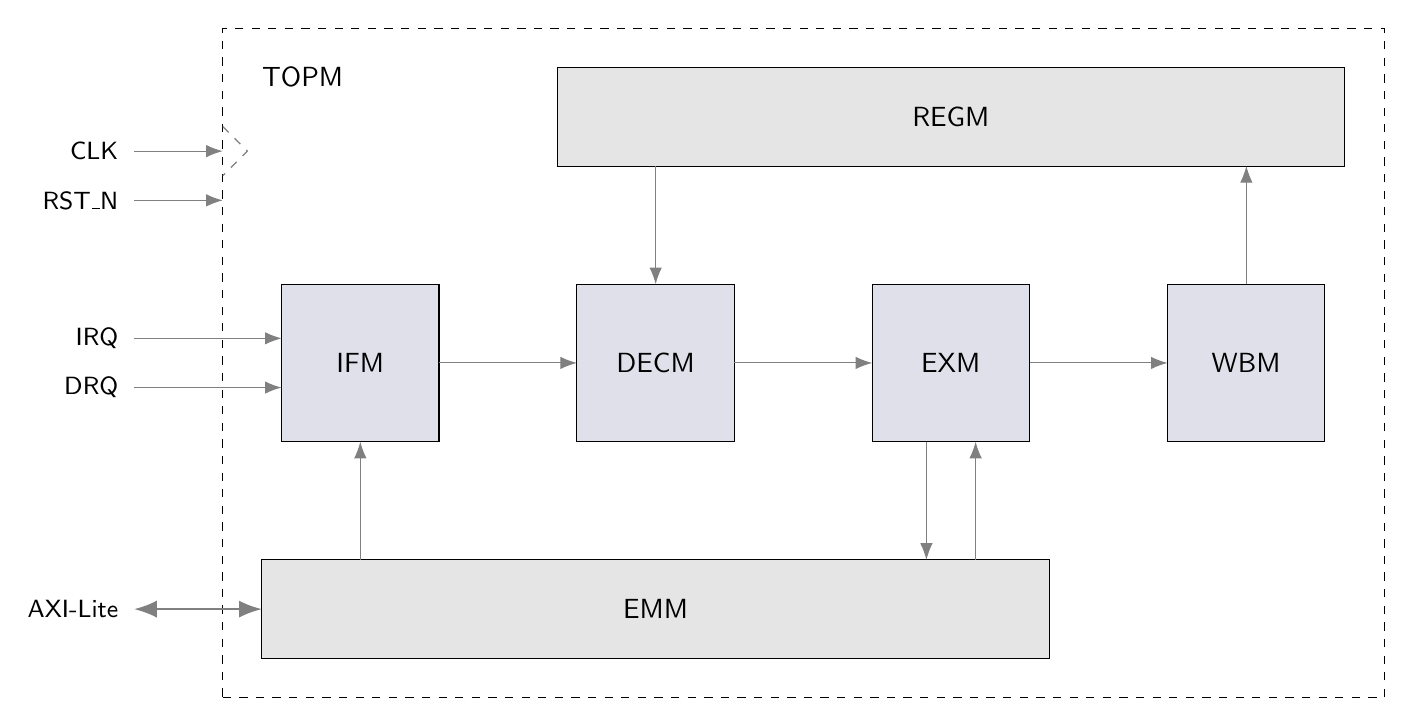
\begin{tikzpicture}[scale=1.25, draw=gray, inner sep=0, outer sep=0]
  \node[rectangle, draw=black,
    minimum height = 1.25cm,
    minimum width = 10cm,
    fill = gray!20] (EMM) at (6, -2.5) {EMM};
  \node[rectangle, draw=black,
    minimum height = 2cm,
    minimum width = 2cm,
    fill = blue!20!gray!20] (IFM) at (3, 0) {IFM};
  \node[rectangle, draw=black,
    minimum height = 2cm,
    minimum width = 2cm,
    fill = blue!20!gray!20] (DECM) at (6, 0) {DECM};
  \node[rectangle, draw=black,
    minimum height = 1.25cm,
    minimum width = 10cm,
    fill = gray!20] (REGM) at (9, 2.5) {REGM};
  \node[rectangle, draw=black,
    minimum height = 2cm,
    minimum width = 2cm,
    fill = blue!20!gray!20] (EXM) at (9, 0) {EXM};
  \node[rectangle, draw=black,
    minimum height = 2cm,
    minimum width = 2cm,
    fill = blue!20!gray!20] (WBM) at (12, 0) {WBM};

  \draw[->] (IFM.east) -- (DECM.west);
  \draw[->] (DECM.east) -- (EXM.west);
  \draw[->] (EXM.east) -- (WBM.west);

  \draw[<-] (IFM.south) -- (IFM.south|- EMM.north);

  \draw[->] ([xshift=-0.25cm]EXM.south) -- ([xshift=-0.25cm]EXM.south |- EMM.north);
  \draw[<-] ([xshift=0.25cm]EXM.south) -- ([xshift=0.25cm]EXM.south |- EMM.north);

  \draw[<-] (DECM.north) -- (DECM.north |- REGM.south);
  \draw[->] (WBM.north) -- (WBM.north |- REGM.south);

  % surrounding rectangle
  \node[dashed, draw=black, align=center, inner sep=0.5cm, fit=(EMM) (IFM) (DECM) (EXM) (WBM) (REGM)] (border) {};
  \node[anchor=north west, inner sep=0.5cm] (border-text) at (border.north west) {TOPM};

  % external interface
  \node (irq) at ([yshift=0.25cm]IFM.west) {};
  \node (drq) at ([yshift=-0.25cm]IFM.west) {};
  \node (axi) at (EMM.west) {};
  \node (clk) at ([yshift=-1.25cm]border.north west) {};
  \node (rst) at ([yshift=-1.75cm]border.north west) {};

  \node (extend) at ([xshift=-1.5cm]irq.center) {};

  \draw[->] (clk.center -| extend.center) node[left=0.2cm, anchor=east]{\small CLK} -- (clk.center);
  \draw[->] (rst.center -| extend.center) node[left=0.2cm, anchor=east]{\small RST\_N} -- (rst.center);
  \draw[->] (irq.center -| extend.center) node[left=0.2cm, anchor=east]{\small IRQ} -- (irq.center);
  \draw[->] (drq.center -| extend.center) node[left=0.2cm, anchor=east]{\small DRQ} -- (drq.center);
  \draw[<->, thick] (axi.center -| extend.center) node[left=0.2cm, anchor=east]{\small AXI-Lite} -- (axi.center);

  % clk triangle
  \draw[-, dashed] ([yshift=0.25cm]clk.center) -- ([xshift=0.25cm]clk.center) -- ([yshift=-0.25cm]clk.center);

\end{tikzpicture}
}

    \caption{Schematic view of the architecture of ECAP5-DPROC}
    \label{fig:architecture}
\end{figure}

  The design is split into the following functional modules :
  \begin{itemize}
    \vspace{-0.5em}
    \item The \textbf{Top Module} (TOPM) which integrates all other modules.
    \item The \textbf{External Memory Module} (EMM), in charge of accessing memory and peripherals.
    \vspace{-0.5em}
    \item The \textbf{Instruction Fetch Module} (IFM), in charge of implementing the instruction fetch stage.
    \vspace{-0.5em}
    \item The \textbf{Decode Module} (DECM), in charge of implementing the decode stage.
    \vspace{-0.5em}
    \item The \textbf{Register Module} (REGM), implementing the internal registers.
    \vspace{-0.5em}
    \item The \textbf{Execute Module} (EXM), in charge of implementing the execute stage.
    \item The \textbf{Write-Back Module} (WBM), in charge of implementing the write-back stage.
  \end{itemize}
\end{content}

\newpage

\section{Top Module}

\begin{content}
  Handshaking and bubbling
\end{content}

\newpage

\section{External Memory Module}
\newpage

\section{Instruction Fetch Module}
\begin{figure}[h!]
    \centering
    \vspace{1em}
\scalebox{0.85}{
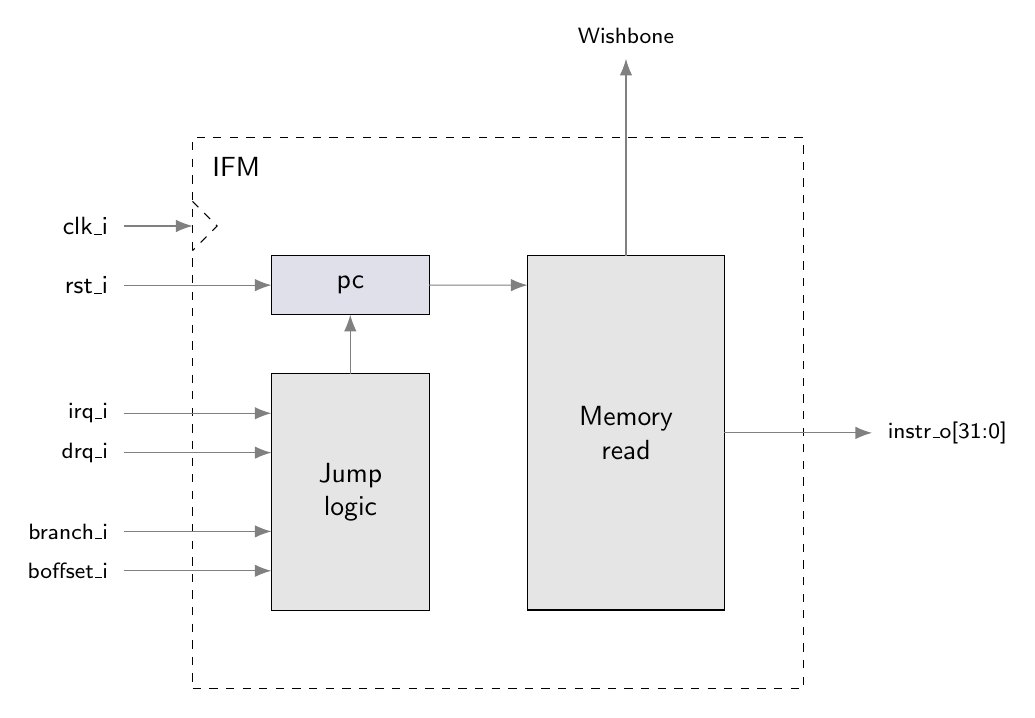
\begin{tikzpicture}[scale=1.25, draw=gray, inner sep=0, outer sep=0]
  \node[rectangle, draw=white,
    minimum height = 5cm,
    minimum width = 2cm] (back) at (0, 0) {};
  \node[rectangle, draw=black,
    anchor=south,
    align=center,
    minimum height = 4.5cm,
    minimum width = 2.5cm,
    fill = gray!20] (mem) at (back.south) {Memory\\read};
  \node[rectangle, draw=black,
    align=center,
    anchor=north east,
    minimum height = 0.75cm,
    minimum width = 2cm,
    fill = blue!20!gray!20] (pc) at ([xshift=-1cm]mem.north west) {pc};
  \node[rectangle, draw=black,
    align=center,
    anchor=south east,
    minimum height = 3cm,
    minimum width = 2cm,
    fill = gray!20] (jmp) at ([xshift=-1cm]mem.south west) {Jump \\ logic};

  \node[dashed, draw=black, align=center, inner sep=1cm, fit=(jmp) (pc) (mem) (back)] (border) {};
  \node[anchor=north west, inner sep=0.25cm] (border-text) at (border.north west) {IFM};

  \node (cross-pc-mem) at (pc.east -| mem.west) {};
  \draw[->] (pc.east) -- (cross-pc-mem.center);

  \draw[->] (jmp.north) -- (pc.south);

  \node (rport1) at (mem.east) {};
  \draw[<-] ([xshift=1.5cm]rport1.center) node[right=0.2cm, anchor=west]{\footnotesize instr\_o[31:0]} -- (rport1.center);

  \node(uport1) at (mem.north) {};
  \draw[<-] ([yshift=2cm]uport1.center) node[above=0.2cm, anchor=south]{\footnotesize Wishbone} -- (uport1.center);

  \node (lport2) at ([yshift=0.4cm]jmp.west) {};
  \node (lport1) at ([yshift=0.4cm]lport2.center) {};
  \node (lport3) at ([yshift=-0.4cm]jmp.west) {};
  \node (lport4) at ([yshift=-0.4cm]lport3.center) {};

  \draw[->] ([xshift=-1.5cm]lport1.center) node[left=0.2cm, anchor=east]{\footnotesize irq\_i} -- (lport1.center);
  \draw[->] ([xshift=-1.5cm]lport2.center) node[left=0.2cm, anchor=east]{\footnotesize drq\_i} -- (lport2.center);
  \draw[->] ([xshift=-1.5cm]lport3.center) node[left=0.2cm, anchor=east]{\footnotesize branch\_i} -- (lport3.center);
  \draw[->] ([xshift=-1.5cm]lport4.center) node[left=0.2cm, anchor=east]{\footnotesize boffset\_i} -- (lport4.center);

  \node (clk) at ([yshift=-0.9cm]border.north west) {};
  \draw[->] ([xshift=-1.5cm]lport3.center |- clk.center) node[left=0.2cm, anchor=east]{\small clk\_i} -- (clk.center);
  % clk triangle
  \draw[-, dashed, draw=black] ([yshift=0.25cm]clk.center) -- ([xshift=0.25cm]clk.center) -- ([yshift=-0.25cm]clk.center);

  \node (rst) at (pc.west) {};
  \draw[->] ([xshift=-1.5cm]rst.center) node[left=0.2cm, anchor=east]{\small rst\_i} -- (rst.center);
\end{tikzpicture}
}

    \caption{Schematic view of the Instruction Fetch Module}
    \label{fig:regm}
\end{figure}

\begin{content}
The instruction fetch module handles fetching from memory the instructions to be executing. The signals are described in table \ref{tab:ifm-interface}. 
\end{content}

{
  \vspace{0.5em}
  \begin{center}
    \refstepcounter{table}
    Table \thetable: Instruction Fetch Module interface signals\label{tab:ifm-interface}
  \end{center}

\footnotesize
\begin{xltabular}{0.9\textwidth}{|l|c|c|X|}
  \hline
  \cellcolor{gray!20}\textbf{NAME} & \cellcolor{gray!20}\textbf{TYPE} & \cellcolor{gray!20}\textbf{WIDTH} & \cellcolor{gray!20}\textbf{DESCRIPTION} \\
  \hline
  clk\_i & I & 1 & Clock input. \\
  \hline
  rst\_i & I & 1 & Reset input. \\
  \hline
  \multicolumn{4}{|l|}{\textbf{JUMP LOGIC}} \\
  \hline
  irq\_i & I & 1 & External interrupt request. \\
  \hline
  drq\_i & I & 1 & External debug request. \\
  \hline
  branch\_i & I & 1 & Branch request. \\
  \hline
  boffset\_i & I & TBC & Branch offset. TBC \\
  \hline
  \multicolumn{4}{|l|}{\textbf{WISHBONE MASTER}} \\
  \hline
  wb\_clk\_o & O & 1 & Wishbone clock output. This is hardwired to clk\_i. \\
  \hline
  wb\_adr\_o & O & 32 & Wishbone read address.  \\
  \hline
  wb\_dat\_i & I & 32 & Wishbone read data. \\
  \hline
  wb\_stb\_o & O & 1 & Strobe output indicates a valid data transfer cycle. \\
  \hline
  wb\_ack\_i & I & 1 & Acknowledge. Indicates a normal termination of a bus cycle. \\
  \hline
  wb\_cyc\_o & O & 1 & Cycle. Indicates that a valid bus cycle is in progress. \\
  \hline
  \multicolumn{4}{|l|}{\textbf{OUTPUT LOGIC}} \\
  \hline
  ready\_i & I & 1 & Asserted when the output is ready to be received. \\
  \hline
  valid\_o & O & 1 & Asserted when the output is ready to be sent. \\
  \hline
  instr\_o & O & 32 & Instruction to be executed. \\
  \hline
\end{xltabular}
}


\begin{content}
  \texttt{pc} stores the value of the next instruction to be loaded from memory. It is connected to the wishbone master which performs the memory read. The read data is transfered to the output logic, in charge of handling the pipeline's handshaking protocol. The value of \texttt{pc} can be either incremented by the output logic, reset by \texttt{rst\_i} or loaded with a specific value through the jump logic.

  This module doesn't contain any prefetch mechanism as there is no performance requirement for revision 1.0.0. This will lead to a performance bottleneck due to the number of cycles needed for fetching instructions from memory.
\end{content}

\subsection{Jump logic}

\begin{figure}[H]
    \centering
    \vspace{1em}
\scalebox{0.85}{
\begin{tikzpicture}[scale=1.25, draw=gray, inner sep=0, outer sep=0]
  \node[rectangle, draw=black,
    align=center,
    anchor=north west,
    minimum height = 4cm,
    minimum width = 3cm,
    fill = gray!20] (jmp) at ([yshift=-0.5cm]pc.south west) {Jump\\logic};

  \node (lport2) at ([yshift=-0.2cm]jmp.west) {};
  \node (lport1) at ([yshift=0.4cm]lport2.center) {};
  \node (lport3) at ([yshift=-0.6cm]lport2.center) {};
  \node (lport4) at ([yshift=-0.4cm]lport3.center) {};

  \draw[->] ([xshift=-1cm]lport1.center) node[left=0.2cm, anchor=east]{\small irq\_i} -- (lport1.center);
  \draw[->] ([xshift=-1cm]lport2.center) node[left=0.2cm, anchor=east]{\small drq\_i} -- (lport2.center);
  \draw[->] ([xshift=-1cm]lport3.center) node[left=0.2cm, anchor=east]{\small branch\_i} -- (lport3.center);
  \draw[->] ([xshift=-1cm]lport4.center) node[left=0.2cm, anchor=east]{\small boffset\_i[]} -- (lport4.center);

  \node (rport2) at ([yshift=0.25cm]jmp.east) {};
  \node (rport1) at ([yshift=-0.5cm]rport2.center) {};
  \draw[<-] ([xshift=1cm]rport1.center) node[right=0.2cm, anchor=west]{\small npc\_o[31:0]} -- (rport1.center);
  \draw[<-] ([xshift=1cm]rport2.center) node[right=0.2cm, anchor=west]{\small pc\_load\_o} -- (rport2.center);
%
  \node (clk) at ([yshift=-0.4cm]jmp.north west) {};
  \draw[->] ([xshift=-1cm]clk.center) node[left=0.2cm, anchor=east]{\small clk\_i} -- (clk.center);
  % clk triangle
  \draw[-, draw=black] ([yshift=0.2cm]clk.center) -- ([xshift=0.2cm]clk.center) -- ([yshift=-0.2cm]clk.center);
%
%  \draw[->] (out.west |- pc.east) -- (pc.east);
\end{tikzpicture}
}

    \caption{Schematic view of the interface of the Jump Logic}
    \label{fig:jump-logic}
\end{figure}

\begin{content}
  The jump logic loads a value into the \texttt{pc} register based on inputs. Its interface is described in table \ref{tab:jump-logic}.
\end{content}

{
  \vspace{0.5em}
  \begin{center}
    \refstepcounter{table}
    Table \thetable: Jump logic interface signals\label{tab:jump-logic}
  \end{center}

\footnotesize
\begin{xltabular}{0.9\textwidth}{|l|c|c|X|}
  \hline
  \cellcolor{gray!20}\textbf{NAME} & \cellcolor{gray!20}\textbf{TYPE} & \cellcolor{gray!20}\textbf{WIDTH} & \cellcolor{gray!20}\textbf{DESCRIPTION} \\
  \hline
  clk\_i & I & 1 & Clock input. \\
  \hline
  irq\_i & I & 1 & External interrupt request. \\
  \hline
  drq\_i & I & 1 & External debug request. \\
  \hline
  branch\_i & I & 1 & Branch request. \\
  \hline
  boffset\_i & I & TBC & Branch offset. TBC \\
  \hline
  pc\_load\_o & O & 1 & Asserted when the pc register shall be updated. \\
  \hline
  npc\_o & O & 32 & Value used to update the pc register. \\
  \hline
\end{xltabular}
}


\begin{content}
\end{content}

\begin{content}
  Figures \ref{fig:jump-logic-behavior} and \ref{fig:jump-logic-output} describe the behavior of the jump logic. The values to be loaded in memory are hardcoded and set at compile time.
\end{content}

\begin{figure}[H]
    \centering
    \vspace{1em}
\scalebox{0.75}{
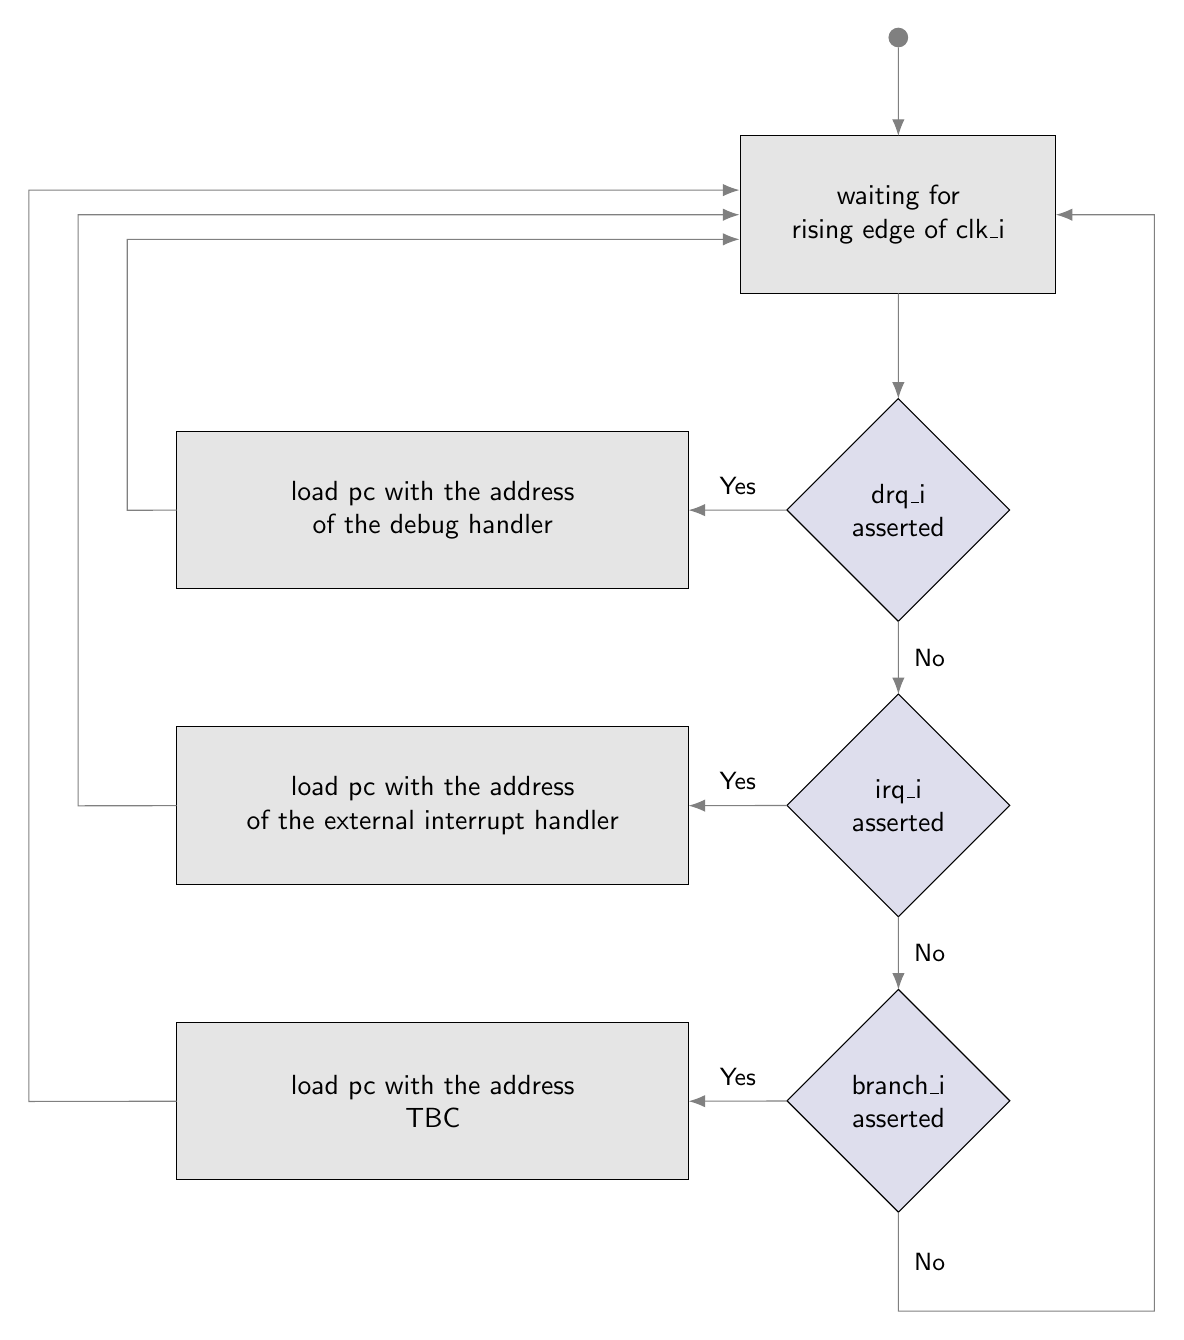
\begin{tikzpicture}[scale=1.25, draw=gray, inner sep=0, outer sep=0]
  \node[rectangle, draw=black,
    align=center,
    anchor=north west,
    minimum height = 2cm,
    minimum width = 4cm,
    fill = gray!20] (box1) at (0, 0) {waiting for\\rising edge of clk\_i};

  \node[rectangle, draw=black,
    minimum height = 2cm,
    minimum width = 2cm,
    rotate=45,
    fill = blue!30!gray!20] (if1) at ([yshift=-3cm]box1.center) {};
  \node[align=center] (if1-text) at (if1.center) {drq\_i\\asserted};

  \node[rectangle, draw=black,
    align=center,
    anchor=east,
    minimum height = 2cm,
    minimum width = 6.5cm,
    fill = gray!20] (box2) at ([xshift=-1cm]if1.north west) {load pc with the address \\ of the debug handler};

  \node[rectangle, draw=black,
    minimum height = 2cm,
    minimum width = 2cm,
    rotate=45,
    fill = blue!30!gray!20] (if2) at ([yshift=-3cm]if1.center) {};
  \node[align=center] (if2-text) at (if2.center) {irq\_i\\asserted};

  \node[rectangle, draw=black,
    align=center,
    anchor=east,
    minimum height = 2cm,
    minimum width = 6.5cm,
    fill = gray!20] (box3) at ([xshift=-1cm]if2.north west) {load pc with the address \\ of the external interrupt handler};

  \node[rectangle, draw=black,
    minimum height = 2cm,
    minimum width = 2cm,
    rotate=45,
    fill = blue!30!gray!20] (if3) at ([yshift=-3cm]if2.center) {};
  \node[align=center] (if3-text) at (if3.center) {branch\_i\\asserted};

  \node[rectangle, draw=black,
    align=center,
    anchor=east,
    minimum height = 2cm,
    minimum width = 6.5cm,
    fill = gray!20] (box4) at ([xshift=-1cm]if3.north west) {load pc with the address \\ TBC};

  \draw[->] (box1.south) -- (if1.north east);
  \draw[->] (if1.south west) -- node[right=0.2cm]{\small No} (if2.north east);
  \draw[->] (if2.south west) -- node[right=0.2cm]{\small No} (if3.north east);

  \draw[->] (if1.north west) -- node[above=0.2cm]{\small Yes} (box2.east);
  \draw[->] (if2.north west) -- node[above=0.2cm]{\small Yes} (box3.east);
  \draw[->] (if3.north west) -- node[above=0.2cm]{\small Yes} (box4.east);

  \node (cross1) at ([yshift=-1cm]if3.south west) {};
  \node (cross2) at ([xshift=1cm]box1.east) {};
  \draw[->] (if3.south west) -- node[right=0.2cm]{\small No} (if3.south west |- cross1.center) -- (cross1.center -| cross2.center) -- (cross2.center) -- (box1.east);

  \node (cross3) at ([xshift=-0.5cm]box2.west) {};
  \node (cross4) at ([xshift=-1cm]box3.west) {};
  \node (cross5) at ([xshift=-1.5cm]box4.west) {};

  \node (cross6) at ([yshift=-0.25cm]box1.west) {};
  \node (cross7) at (box1.west) {};
  \node (cross8) at ([yshift=0.25cm]box1.west) {};

  \draw[->] (box2.west) -- (cross3.center) -- (cross3.center |- cross6.west) -- (cross6.west);
  \draw[->] (box3.west) -- (cross4.center) -- (cross4.center |- cross7.west) -- (cross7.west);
  \draw[->] (box4.west) -- (cross5.center) -- (cross5.center |- cross8.west) -- (cross8.west);

  \node [circle, fill=gray, minimum height = 0.25cm, minimum width = 0.25cm] (start) at ([yshift=1cm]box1.north) {};
  \draw[->] (start.south) -- (box1.north) {};
\end{tikzpicture}
}

    \caption{Activity diagram of the jump logic behavior}
    \label{fig:jump-logic-behavior}
\end{figure}

\begin{figure}[H]
    \centering
    \begin{tikztimingtable}[%
    scale=0.9,
    timing/dslope=0.1,
    timing/.style={x=5ex,y=3ex},
    x=5ex,
    timing/rowdist=5ex,
    timing/name/.style={font=\footnotesize},
    timing/u/background/.style={fill=gray!20},
    timing/e/background/.style={fill=gray!20},
]

clk\_i & H 3{C C} L \\
npc\_o & 2U 2D{new pc value} 4U  \\
pc\_load\_o & 2L 0.2E 1.8H 0.2E 4L \\
pc & 4D{previous pc value} 4D{new pc value} \\
\extracode
% grid
\begin{pgfonlayer}{background}
\begin{scope}[semitransparent ,semithick]
\vertlines[darkgray,dotted]{2, 4, 6}
\end{scope}
\end{pgfonlayer}
\end{tikztimingtable}

    \caption{Timing diagram for the output port of the jump logic.}
    \label{fig:jump-logic-output}
\end{figure}

\subsection{PC register}

\begin{figure}[H]
    \centering
    \vspace{1em}
\scalebox{0.75}{
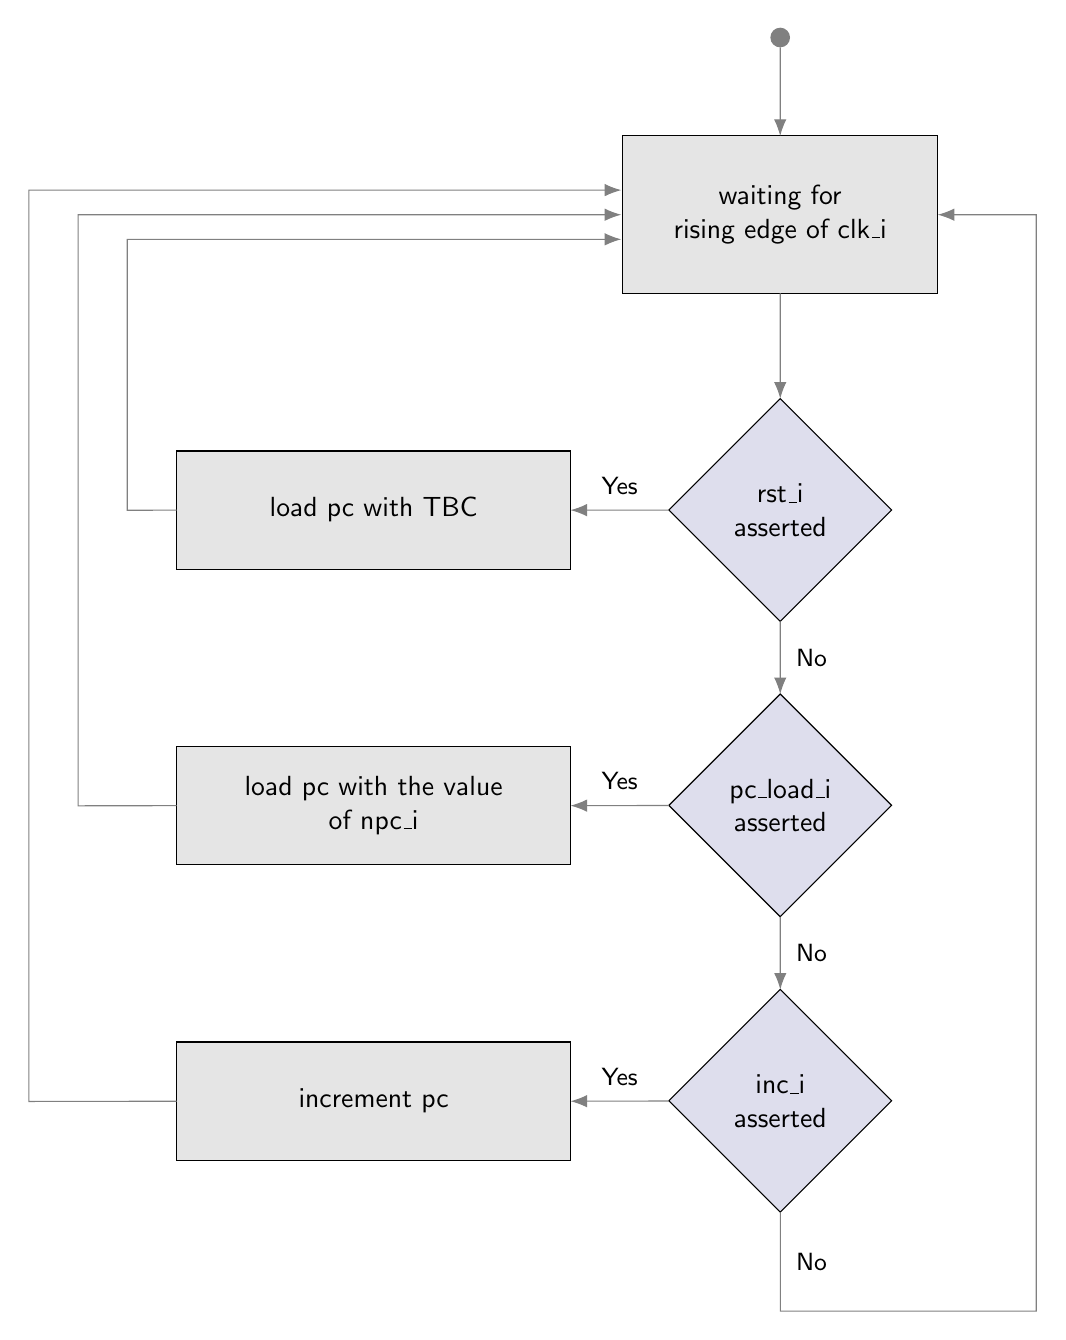
\begin{tikzpicture}[scale=1.25, draw=gray, inner sep=0, outer sep=0]
  \node[rectangle, draw=black,
    align=center,
    anchor=north west,
    minimum height = 2cm,
    minimum width = 4cm,
    fill = gray!20] (box1) at (0, 0) {waiting for\\rising edge of clk\_i};

  \node[rectangle, draw=black,
    minimum height = 2cm,
    minimum width = 2cm,
    rotate=45,
    fill = blue!30!gray!20] (if1) at ([yshift=-3cm]box1.center) {};
  \node[align=center] (if1-text) at (if1.center) {rst\_i\\asserted};

  \node[rectangle, draw=black,
    align=center,
    anchor=east,
    minimum height = 1.5cm,
    minimum width = 5cm,
    fill = gray!20] (box2) at ([xshift=-1cm]if1.north west) {load pc with TBC};

  \node[rectangle, draw=black,
    minimum height = 2cm,
    minimum width = 2cm,
    rotate=45,
    fill = blue!30!gray!20] (if2) at ([yshift=-3cm]if1.center) {};
  \node[align=center] (if2-text) at (if2.center) {pc\_load\_i\\asserted};

  \node[rectangle, draw=black,
    align=center,
    anchor=east,
    minimum height = 1.5cm,
    minimum width = 5cm,
    fill = gray!20] (box3) at ([xshift=-1cm]if2.north west) {load pc with the value \\ of npc\_i};

  \node[rectangle, draw=black,
    minimum height = 2cm,
    minimum width = 2cm,
    rotate=45,
    fill = blue!30!gray!20] (if3) at ([yshift=-3cm]if2.center) {};
  \node[align=center] (if3-text) at (if3.center) {inc\_i\\asserted};

  \node[rectangle, draw=black,
    align=center,
    anchor=east,
    minimum height = 1.5cm,
    minimum width = 5cm,
    fill = gray!20] (box4) at ([xshift=-1cm]if3.north west) {increment pc};

  \draw[->] (box1.south) -- (if1.north east);
  \draw[->] (if1.south west) -- node[right=0.2cm]{\small No} (if2.north east);
  \draw[->] (if2.south west) -- node[right=0.2cm]{\small No} (if3.north east);

  \draw[->] (if1.north west) -- node[above=0.2cm]{\small Yes} (box2.east);
  \draw[->] (if2.north west) -- node[above=0.2cm]{\small Yes} (box3.east);
  \draw[->] (if3.north west) -- node[above=0.2cm]{\small Yes} (box4.east);

  \node (cross1) at ([yshift=-1cm]if3.south west) {};
  \node (cross2) at ([xshift=1cm]box1.east) {};
  \draw[->] (if3.south west) -- node[right=0.2cm]{\small No} (if3.south west |- cross1.center) -- (cross1.center -| cross2.center) -- (cross2.center) -- (box1.east);

  \node (cross3) at ([xshift=-0.5cm]box2.west) {};
  \node (cross4) at ([xshift=-1cm]box3.west) {};
  \node (cross5) at ([xshift=-1.5cm]box4.west) {};

  \node (cross6) at ([yshift=-0.25cm]box1.west) {};
  \node (cross7) at (box1.west) {};
  \node (cross8) at ([yshift=0.25cm]box1.west) {};

  \draw[->] (box2.west) -- (cross3.center) -- (cross3.center |- cross6.west) -- (cross6.west);
  \draw[->] (box3.west) -- (cross4.center) -- (cross4.center |- cross7.west) -- (cross7.west);
  \draw[->] (box4.west) -- (cross5.center) -- (cross5.center |- cross8.west) -- (cross8.west);

  \node [circle, fill=gray, minimum height = 0.25cm, minimum width = 0.25cm] (start) at ([yshift=1cm]box1.north) {};
  \draw[->] (start.south) -- (box1.north) {};
\end{tikzpicture}
}

    \caption{Activity diagram of the pc register}
    \label{fig:pc-behavior}
\end{figure}

\subsection{Wishbone master}

\begin{figure}[H]
    \centering
    \vspace{1em}
\scalebox{0.85}{
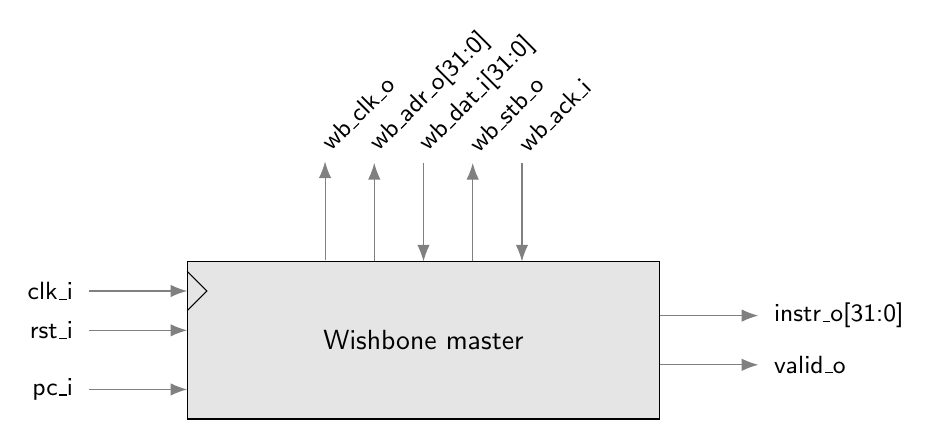
\begin{tikzpicture}[scale=1.25, draw=gray, inner sep=0, outer sep=0]
  \node[rectangle, draw=black,
    anchor=south,
    align=center,
    minimum height = 2cm,
    minimum width = 6cm,
    fill = gray!20] (mem) at (0, 0) {Wishbone master};

  \node(uport4) at ([xshift=0.5cm]mem.north) {};
  \node(uport3) at ([xshift=-0.5cm]uport4.center) {};
  \node(uport2) at ([xshift=-0.5cm]uport3.center) {};
  \node(uport1) at ([xshift=-0.5cm]uport2.north) {};
  \node(uport5) at ([xshift=0.5cm]uport4.center) {};
  \draw[<-] ([yshift=1cm]uport1.center) node[above=0.2cm, anchor=west, rotate=45]{\small wb\_clk\_o} -- (uport1.center);
  \draw[<-] ([yshift=1cm]uport2.center) node[above=0.2cm, anchor=west, rotate=45]{\small wb\_adr\_o[31:0]} -- (uport2.center);
  \draw[->] ([yshift=1cm]uport3.center) node[above=0.2cm, anchor=west, rotate=45]{\small wb\_dat\_i[31:0]} -- (uport3.center);
  \draw[<-] ([yshift=1cm]uport4.center) node[above=0.2cm, anchor=west, rotate=45]{\small wb\_stb\_o} -- (uport4.center);
  \draw[->] ([yshift=1cm]uport5.center) node[above=0.2cm, anchor=west, rotate=45]{\small wb\_ack\_i} -- (uport5.center);

  \node(lport1) at ([yshift=-0.5cm]mem.west) {};
  \draw[->] ([xshift=-1cm]lport1.center) node[left=0.2cm, anchor=east]{\small pc\_i} -- (lport1.center);

  \node(rport1) at ([yshift=0.25cm]mem.east) {};
  \node(rport2) at ([yshift=-0.5cm]rport1.center) {};
  \draw[<-] ([xshift=1cm]rport1.center) node[right=0.2cm, anchor=west]{\small instr\_o[31:0]} -- (rport1.center);
  \draw[<-] ([xshift=1cm]rport2.center) node[right=0.2cm, anchor=west]{\small valid\_o} -- (rport2.center);

  \node (clk) at ([yshift=-0.3cm]mem.north west) {};
  \draw[->] ([xshift=-1cm]clk.center) node[left=0.2cm, anchor=east]{\small clk\_i} -- (clk.center);
  % clk triangle
  \draw[-, draw=black] ([yshift=0.2cm]clk.center) -- ([xshift=0.2cm]clk.center) -- ([yshift=-0.2cm]clk.center);

  \node (rst) at ([yshift=-0.4cm]clk.center) {};
  \draw[->] ([xshift=-1cm]rst.center) node[left=0.2cm, anchor=east]{\small rst\_i} -- (rst.center);
\end{tikzpicture}
}

    \caption{Schematic view of the interface of the Wishbone Master}
    \label{fig:ifm-wishbone-master}
\end{figure}

\begin{content}
  The wishbone master fetches from memory the instruction to be executed. Its interface is described in table \ref{tab:ifm-wishbone-master}.
\end{content}

{
  \vspace{0.5em}
  \begin{center}
    \refstepcounter{table}
    Table \thetable: Instruction Fetch Module interface signals\label{tab:ifm-wishbone-master}
  \end{center}

\footnotesize
\begin{xltabular}{0.9\textwidth}{|l|c|c|X|}
  \hline
  \cellcolor{gray!20}\textbf{NAME} & \cellcolor{gray!20}\textbf{TYPE} & \cellcolor{gray!20}\textbf{WIDTH} & \cellcolor{gray!20}\textbf{DESCRIPTION} \\
  \hline
  clk\_i & I & 1 & Clock input. \\
  \hline
  rst\_i & I & 1 & Reset input. \\
  \hline
  \multicolumn{4}{|l|}{\textbf{WISHBONE MASTER}} \\
  \hline
  wb\_clk\_o & O & 1 & Wishbone clock output. This is hardwired to clk\_i. \\
  \hline
  wb\_adr\_o & O & 32 & Wishbone read address.  \\
  \hline
  wb\_dat\_i & I & 32 & Wishbone read data. \\
  \hline
  wb\_stb\_o & O & 1 & Strobe output indicates a valid data transfer cycle. \\
  \hline
  wb\_ack\_i & I & 1 & Acknowledge. Indicates a normal termination of a bus cycle. \\
  \hline
  \multicolumn{4}{|l|}{\textbf{OUTPUT}} \\
  \hline
  instr\_o & O & 32 & Instruction to be executed. \\
  \hline
  valid\_o & O & 1 & Asserted when the instruction output is valid. \\
  \hline
\end{xltabular}
}


\subsection{Output logic}

\newpage
\section{Decode Module}
\newpage

\section{Register Module}

\begin{figure}[h!]
    \centering
    \vspace{1em}
\scalebox{0.85}{
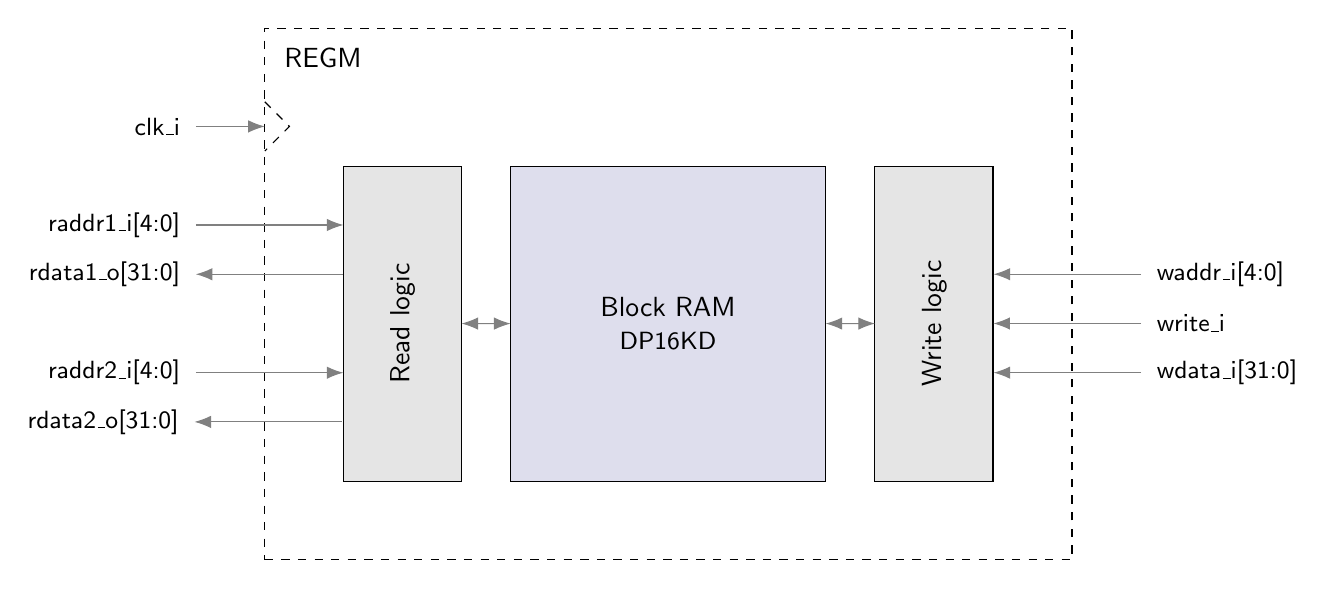
\begin{tikzpicture}[scale=1.25, draw=gray, inner sep=0, outer sep=0]
  \node[rectangle, draw=white,
    align=center,
    minimum height = 4.75cm,
    minimum width = 4cm,
    fill = white] (back) at (6, 2.5) {Block RAM \\ \small DP16KD};
  \node[rectangle, draw=black,
    align=center,
    anchor=south,
    minimum height = 4cm,
    minimum width = 4cm,
    fill = blue!30!gray!20] (BRAM) at (back.south) {Block RAM \\ \small DP16KD};

  \node[rectangle, draw=black,
    align=center,
    anchor=east,
    minimum height = 4cm,
    minimum width = 1.5cm,
    fill = gray!20] (glue1) at ([xshift=-0.5cm]BRAM.west) {};
  \node[rotate=90] (glue1text) at (glue1.center) {Read logic};

  \node[rectangle, draw=black,
    align=center,
    anchor=west,
    minimum height = 4cm,
    minimum width = 1.5cm,
    fill = gray!20] (glue2) at ([xshift=0.5cm]BRAM.east) {};
  \node[rotate=90] (glue2text) at (glue2.center) {Write logic};

  \node[dashed, draw=black, align=center, inner sep=1cm, fit=(BRAM) (back) (glue1) (glue2)] (border) {};
  \node[anchor=north west, inner sep=0.25cm] (border-text) at (border.north west) {REGM};

  \node (lport2) at ([yshift=0.5cm]glue1.west) {};
  \node (lport1) at ([yshift=0.5cm]lport2.center) {};
  \draw[->] ([xshift=-1.5cm]lport1.center) node[left=0.2cm, anchor=east]{\small raddr1\_i[4:0]} -- (lport1.center);
  \draw[<-] ([xshift=-1.5cm]lport2.center) node[left=0.2cm, anchor=east]{\small rdata1\_o[31:0]} -- (lport2.center);

  \node (lport3) at ([yshift=-0.5cm]glue1.west) {};
  \node (lport4) at ([yshift=-0.5cm]lport3.west) {};
  \draw[->] ([xshift=-1.5cm]lport3.center) node[left=0.2cm, anchor=east]{\small raddr2\_i[4:0]} -- (lport3.center);
  \draw[<-] ([xshift=-1.5cm]lport4.center) node[left=0.2cm, anchor=east]{\small rdata2\_o[31:0]} -- (lport4.center);

  \node (rport2) at (glue2.east) {};
  \node (rport1) at ([yshift=0.5cm]rport2.center) {};
  \node (rport3) at ([yshift=-0.5cm]rport2.center) {};
  \draw[->] ([xshift=1.5cm]rport1.center) node[right=0.2cm, anchor=west]{\small waddr\_i[4:0]} -- (rport1.center);
  \draw[->] ([xshift=1.5cm]rport2.center) node[right=0.2cm, anchor=west]{\small write\_i} -- (rport2.center);
  \draw[->] ([xshift=1.5cm]rport3.center) node[right=0.2cm, anchor=west]{\small wdata\_i[31:0]} -- (rport3.center);

  \node (clk) at ([yshift=-1cm]border.north west) {};
  \draw[->] ([xshift=-1.5cm]lport3.center |- clk.center) node[left=0.2cm, anchor=east]{\small clk\_i} -- (clk.center);
  % clk triangle
  \draw[-, dashed, draw=black] ([yshift=0.25cm]clk.center) -- ([xshift=0.25cm]clk.center) -- ([yshift=-0.25cm]clk.center);

  \draw[<->] (glue1.east) -- (BRAM.west);
  \draw[<->] (glue2.west) -- (BRAM.east);
\end{tikzpicture}
}

    \caption{Schematic view of the Register Module}
    \label{fig:regm}
\end{figure}

\begin{content}
The register module implements the 32 internal registers of ECAP5-DPROC. It has two reading port and one writing port. The signals are described in table \ref{tab:regm-interface}. 
\end{content}

\begin{table}[H]
  \centering
  {
\footnotesize
\begin{tabularx}{0.9\textwidth}{|l|c|c|X|}
  \hline
  \cellcolor{gray!20}\textbf{NAME} & \cellcolor{gray!20}\textbf{TYPE} & \cellcolor{gray!20}\textbf{WIDTH} & \cellcolor{gray!20}\textbf{DESCRIPTION} \\
  \hline
  clk\_i & I & 1 & Clock input. \\
  \hline
  \multicolumn{4}{|l|}{\textbf{FIRST READING PORT}} \\
  \hline
  raddr1\_i & I & 5 & Register selector. \\
  \hline
  rdata1\_o & O & 32 & Selected register value. \\
  \hline
  \multicolumn{4}{|l|}{\textbf{SECOND READING PORT}} \\
  \hline
  raddr2\_i & I & 5 & Register selector. \\
  \hline
  rdata2\_o & O & 32 & Selected register value. \\
  \hline
  \multicolumn{4}{|l|}{\textbf{WRITING PORT}} \\
  \hline
  waddr\_i & I & 5 & Register selector. \\
  \hline
  write\_i & I & 1 & Asserted to indicate a write. \\
  \hline
  wdata\_i & I & 32 & Data to be written. \\
  \hline
\end{tabularx}
}

  \caption{Register Module interface signals}
  \label{tab:regm-interface}
\end{table}

\begin{content}
  When reading, \texttt{rdata1\_i} and \texttt{rdata2\_i} output, on the rising edge of \texttt{clk\_i}, the value of the register respectively selected by \texttt{raddr1\_i} and \texttt{raddr2\_i}. A register write happens on the rising edge of \texttt{clk\_i} when \texttt{write\_i} is asserted, writing the value \texttt{wdata\_i} in the register selected by \texttt{waddr\_i}.
\end{content}

\newpage

\section{Execute Module}
\newpage

\section{Write-Back Module}
\newpage

\section{Debug}
\newpage


\end{document}
